
\section[Continuous Integration]{Continuous Integration}

\subsection[]{Continuous Integration}
\begin{frame}
\frametitle{Continuous Integration}
\begin{itemize}%TODO try include quote
	\item Definition by Martin Fowler:
		\begin{itemize}
		\item \emph{“Continuous Integration is a software development practice where members of a team integrate their work frequently, usually \textbf{each person integrates at least daily} - leading to multiple integrations per day. Each integration is \textbf{verified by an automated build (including test)} to detect integration errors as quickly as possible.”}
		\end{itemize}
	\item Team of developers integrate and test their code early and often.
	\item Reduce the risk of seeing “integration hell”.
	\item Automated testing is a key part of Continuous Integration.
	\item Address the conflicts and issues early.
	\item Get fast feedback on code changes.
\end{itemize}
\end{frame}

\subsection[]{11 Practices by Martin Fowler}
\begin{frame}
\frametitle{11 Practices by Martin Fowler}
\begin{enumerate}
	\item Maintain a Single Source Repository.
	\item Automate the Build
	\item Make Your Build Self-Testing
	\item Everyone Commits To the Mainline Every Day
	\item Every Commit Should Build the Mainline on an Integration Machine
	\item Fix Broken Builds Immediately
	\item Keep the Build Fast
	\item Test in a Clone of the Production Environment
	\item Make it Easy for Anyone to Get the Latest Executable
	\item Everyone can see what's happening
	\item Automate Deployment
\end{enumerate}
\end{frame}


\subsection[]{Typical Issues}
\begin{frame}
\frametitle{Typical Issues}
\begin{itemize}
	\item Builds fails too often.
	\item Developers are not able to verify the code before commit.
	\item Test engineers are waiting too long to get new version.
	\item Single step of build pipeline cannot be repeated.
	\item Number of muted tests is growing.
	\item It’s hard to identify source of the issue – single build contains a lot of changes.
\end{itemize}
\end{frame}

\subsection[]{Improvements}
\begin{frame}
\frametitle{Improvements}
\begin{itemize}
	\item Automate everything that can be automated (build, environment preparation, tests etc.).
	\item Let developers to run all validation steps locally.
	\item Isolate each build step and make it standalone.
	\item Split monolithic build into smaller build configurations.
	\item Execute some of the build steps in parallel (e.g. tests and package preparation).
	\item Scale build configurations: Fast/Common/Nightly
\end{itemize}
\end{frame}

\subsection[]{Continuous Delivery and Deployment}
\begin{frame}
\frametitle{Continuous Delivery and Deployment}
\begin{itemize}
	\item \textbf{Continuous Delivery}
		\begin{itemize}%quote?
		\item Definition by Martin Fowler:
			\begin{itemize}
			\item \emph{“Continuous Delivery is a software development discipline where you build software in such a way that the \textbf{software can be released} to production at any time.”} by Martin Fowler
			\end{itemize}
		\item Exists on top of Continues Integration.
		\item Deployment and release process automated.
		\item Every change \textbf{can be deployed} to production but you may choose not to do it because of business priorities.
		\end{itemize}
	\item \textbf{Continuous Deployment}
		\begin{itemize}
		\item Sometimes confused with Continuous Delivery but goes one step further.
		\item Every change that passes all stages of the production pipeline is released to customers.
		\end{itemize}
\end{itemize}
\end{frame}

\begin{frame}
\frametitle{Continuous Delivery and Deployment}
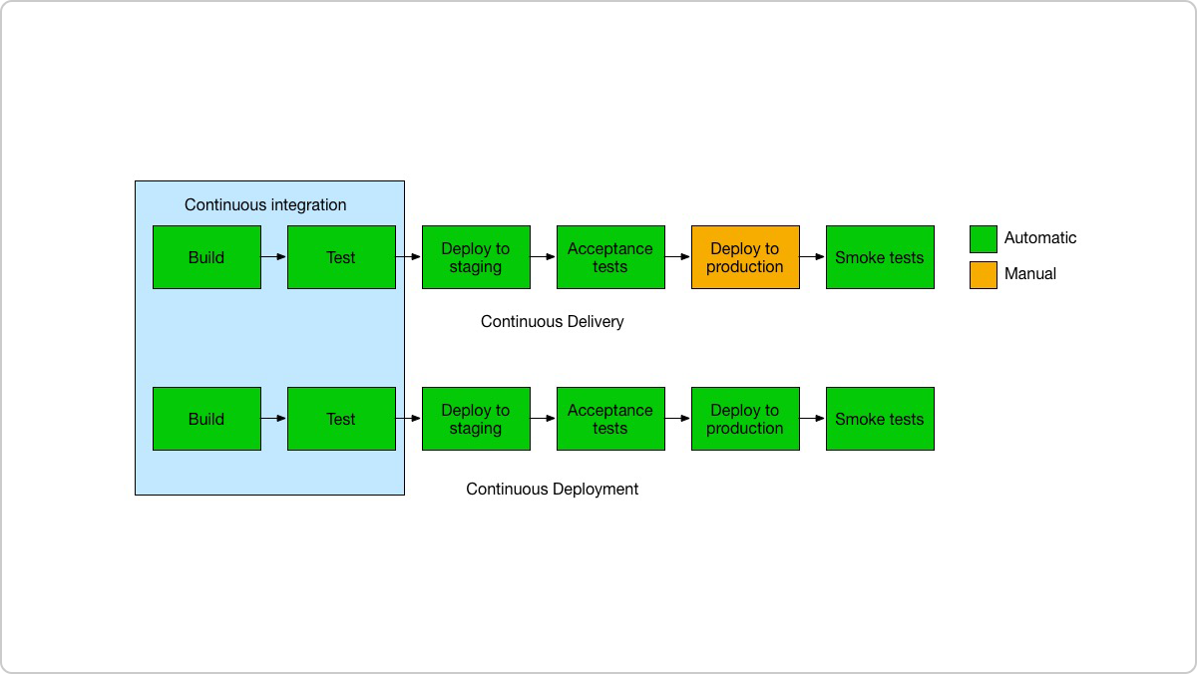
\includegraphics[width=\textwidth, height=0.56\textwidth]{cont-delivery-deployment.png}
\end{frame}

\begin{frame}
\frametitle{Tools Overview}
\begin{itemize}
	\item Jenkins
	\item TeamCity
	\item GitLab CI/CD
	\item Bamboo
	\item Bitbucket Pipelines
\end{itemize}
\end{frame}
